\section{Versuchsaufbau}
\label{sec:Versuchaufbau}

Zur Erzeugung der Röntgenstrahlung wird eine Cu-Röntgenröhre verwendet. Die
Beschleunigungsspannung beträgt stets $35\si{\kilo\volt}$, der Emissionsstrom
beträgt $1\si{\milli\ampere}$. Abbildung \ref{fig:Aufbau} zeigt den Aufbau des
Experiments.
\begin{figure}
  \centering
  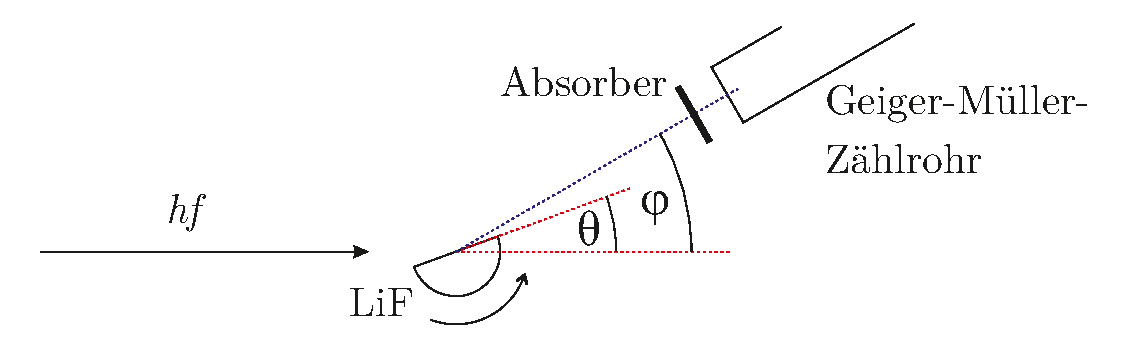
\includegraphics[width=0.9\textwidth]{ressources/Aufbau.pdf}
  \caption{Schematischer Aufbau des Experiments.}
  \label{fig:Aufbau}
\end{figure}
Die in der Röntgenröhre generierte Strahlung trifft auf einen LiF-Kristall mit
Gitterkonstante $d=201,4\si{\pico\meter}$. Dieser kann um einen Winkel $\Theta$
rotiert werden. Ebenso kann der Detektor samt Absorber um einen Winkel $\phi$
rotiert werden. Dabei existiert die Möglichkeit, den Winkel $\phi$ fest auf das doppelte des Winkels $\Theta$ einzustellen, sodass stets das Intensitätsmaximum beobachtet wird. Der Detektor ist ein Geiger-Müller-Zählrohr und als Absorber stehen verschiedene Elemente zur Verfügung.
